\documentclass[12pt]{article}
\usepackage{polski}
\usepackage[utf8]{inputenc}
\usepackage{fullpage}
\usepackage{tabto}
\usepackage{graphicx} 
\usepackage{float}
\usepackage{caption}
\usepackage{indentfirst} 
\usepackage[table,xcdraw]{xcolor}


% zmienić copena na cohena i jeżeli jest capa ma byc cappa
% biblio źle wyglada
% poprawić te tabelki w macierzach konfuzji
% 4 pierwsze rozdzialy sa gotowe, przeczytac i poprawic ewentualne bledy

\linespread{1.3}
\begin{document}
%---------------------------------------------------------
%					Strona Tytułowa
%---------------------------------------------------------
\begin{titlepage}
%-----------------------Tytuł-----------------------------
\newcommand{\LINE}{\rule{\linewidth}{0.7mm}}
\center
\LINE \\[0.5cm]
\Large\textsc{Komputerowe wspomaganie diagnozowania nowotworów piersi z wykorzystaniem algorytmów minimalno-odległościowych}\\ [5mm]
\normalsize\textsc{Zastosowanie Informatyki w Medycynie}  \\[0.5cm]
\LINE \\[3cm]
%----------------------Nazwiska---------------------------
\begin{minipage}{0.5\textwidth}
\begin{flushleft} \large
\emph{Autorzy:}
		\\Mateusz Ożóg %226125
		\\Grzegorz Milaszkiewicz %226110
\end{flushleft}
\end{minipage}
~
\begin{minipage}{0.45\textwidth}
\begin{flushright} \large
\emph{Prowadzący:} \\
mgr inż. Jakub Klikowski
\end{flushright}
\end{minipage}\\[2cm]
%----------------------Stopka-----------------------------
\vfill
\center Wrocław 2019
\end{titlepage}

%---------------------------------------------------------
%					Spis treści
%---------------------------------------------------------
\renewcommand{\contentsname}{Spis treści}
\tableofcontents
\newpage

%---------------------------------------------------------
%					Część pierwsza
%---------------------------------------------------------
\section{Charakterystyka analizowanego problemu}
Tematem naszego projektu jest wspomniane w tytule, komputerowe wspomaganie diagnozowania nowotworów piersi przy pomocy algorytmów minimalno-odległościowych. Na podstawie empirycznego materiału diagnostycznego należało zbadać poprawność diagnoz losowo wybranych pacjentów dla zaimplementowanych mechanizmów rozpoznawania.
\newline
\indent Pojedyncza diagnoza przyporządkowuje pacjentkę do jednej z wyodrębnionych klas. Przeprowadzana jest na podstawie pewnych cech, które ją charakteryzują (parametry badań). Poszczególne klasy posiadają charakterystyczne wartości wyróżnionych właściwości. W procesie rozpoznawania każdy z parametrów pomaga określić przynależność do danego zbioru. Wartości niektórych z nich mogą jednoznacznie determinować klasę danego pacjenta, natomiast inne tylko ją zasugerować. W związku z tym przeprowadzono ranking cech, który posortował poszczególne parametry, zgodnie z ich znaczeniem w procesie rozpoznawania. 
\newline \indent Dla ułatwienia zrozumienia problemu i dokonania jego dokładniejszej analizy, poniżej przedstawiono krótką analizę danych poddawanych późniejszym procesom rozpoznawania.


\subsection{Analiza materiału diagnostycznego}
\indent Do badania przystąpiło 569 kobiet, u których został zdiagnozowany rak piersi. Każda z nich została opisana za pomocą 32 wartości. Pierwsza jest numerem identyfikacyjnym, druga składa się z dwóch liter M lub B i oznacza przynależność do danej klasy.  Grupa z rakiem łagodnym (357 kobiet) oznaczona jest literą B, natomiast z rakiem złośliwym (212 kobiet) literą M. Rozkład ilości pacjentów przynależnych do danych klas przedstawiony został na rysunku \ref{przynaleznosc_pacjentek} (malignant - nowotwór złośliwy, benign - nowotwór łagodny). Pozostałe wartości, w liczbie 30, wyznaczane były na podstawie wyglądu jądra komórkowego każdej z pacjentek.
\newline

\begin{figure}[H]
	\centering
		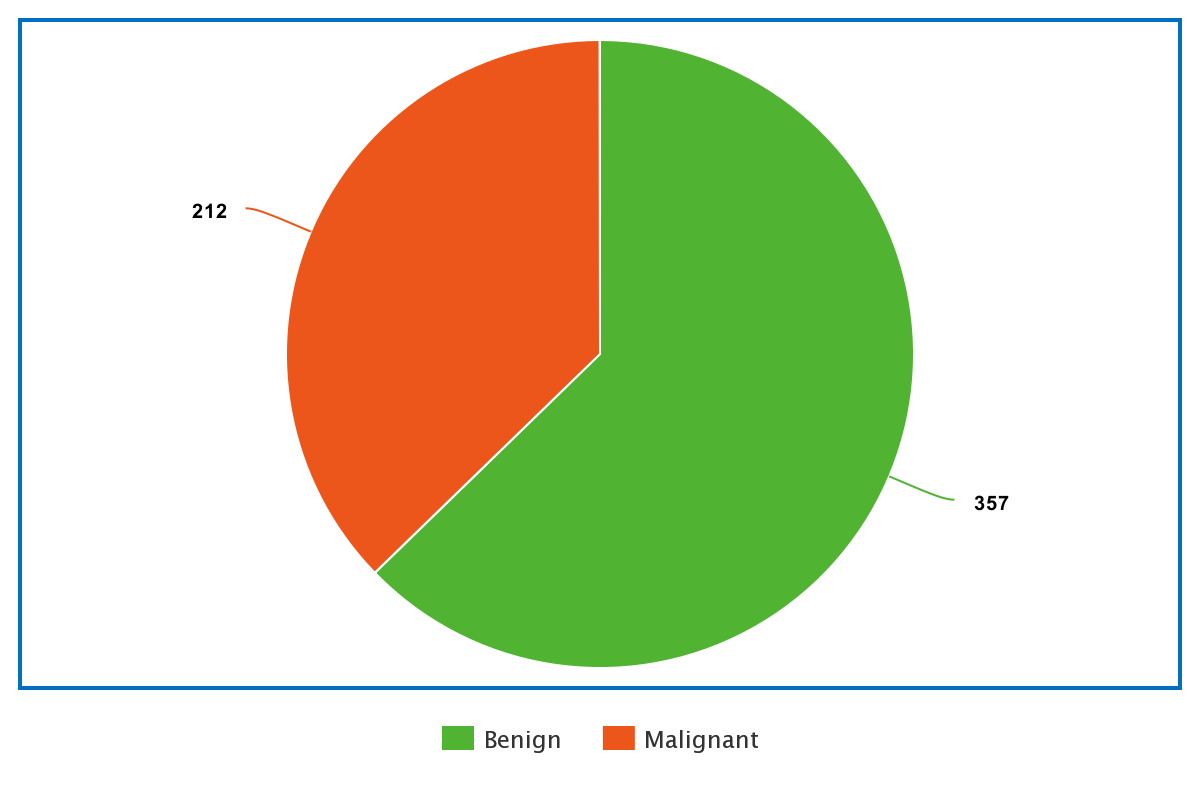
\includegraphics[scale=0.6]{images/pie_chart.png}
	\caption{Przynależność pacjentek do wyznaczonych klas}
	\label{przynaleznosc_pacjentek}
\end{figure}

\indent U każdej z kobiet zostało wyróżnionych 10 cech głównych (tabela \ref{cechy}) oraz 20 dodatkowych opisujących błąd standardowy oraz najgorszą uzyskaną wartość dla każdej z nich. Co razem daje 30 cech. 
\newline

\begin{table}[H]
\captionof{table}{Cechy jądra komórkowego wykorzystywane w procesie rozpoznawania} 
\label{cechy}
	\begin{tabular}{|p{0.2\linewidth}|p{0.74\linewidth}|}%{|l|l|}
	\hline\centering
	Numer cechy 	& Opis 				\\ \hline\centering
	1	& Promień (średnia odległość od środka do punktów na obwodzie) \\ \hline\centering
	2	& Tekstura (odchylenie standardowe wartości skali szarości) \\ \hline\centering
	3	& Obwód \\ \hline\centering
	4	& Powierzchnia \\ \hline\centering
	5	& Gładkość \\ \hline\centering
	6	& Ścisłość(obwód$^2/powierzchnia-1.0$) \\ \hline\centering
	7	& Wklęsłość (dotkliwość wklęsłych części konturu) \\ \hline\centering
	8	& Wklęsłe punkty (liczba wklęsłych części konturu) \\ \hline\centering
	9	& Symetria \\ \hline\centering
	10	& Wymiar fraktalny ("przybliżenie linii brzegowej" - 1) \\ \hline
	\end{tabular}
\end{table}
\indent Podsumowując analizę przedstawionego problemu rozpoznawania, pacjentów z grupy testowej będziemy przyporządkowywać do jednej z dwóch klas. Więcej informacji empirycznej posiadamy na temat klasy reprezentującej nowotwór łagodny, co jest spowodowane większą liczbą kobiet w jego gronie. Każda z pacjentek posiada 30 cech, które przedstawione są za pomocą wielowartościowych liczb rzeczywistych. Pojedyncza cecha z pewną dokładnością wyznacza klasyfikację do danej grupy. W celu uzyskania dokładniejszych wyników w procesie rozpoznawania będziemy przeprowadzali ranking cech, wykorzystując kryterium Kołmogorova-Smirnova, które porządkuje parametry pacjentów rozpoczynając od cech o największym znaczeniu. Sam proces rozpoznawania opierać się będzie na implementacji klasyfikatorów minimalno-odległościowych tj. NM (nearest mean), NN (nearest neighbour) oraz KNN (k-nearest neighbours).

%---------------------------------------------------------
%					Część druga
%---------------------------------------------------------
\section{Opis stosowanych algorytmów}

\indent W procesie klasyfikacji pacjentów do poszczególnych klas zostaną wykorzystane algorytmy: najbliższej średniej oraz k-najbliższych sąsiadów. W przypadku drugiego algorytmu jako parametr k (ilość sąsiadów) zostaną przyjęte następujące wartości: 1 (najbliższy sąsiad), 5 oraz 9. Pacjentów będziemy dzielić na 2 grupy. Zbiór uczący będzie określał obiekty z zdiagnozowaną klasą. W zbiorze testowym natomiast będą znajdowali się pacjenci poddawani klasyfikacji na podstawie przetworzonych danych z grupy uczącej. Struktura danych w obu algorytmach jest identyczna. Każdy pacjent będzie określany za pomocą wektora cech tak jak to przedstawiono we wzorze poniżej.
\begin{center}
\[ \vec{X} = (x_1, x_2, ... , x_n)\]
\end{center}


Każdy zbiór będzie składał się z m takich wektorów, gdzie m oznacza liczbę przypisanych do niego pacjentów. Litera y oznacza przynależność do jednej z wyszczególnionych klas dla i-tego pacjenta (litera 'M' bądź 'B').
Zbiory uczące i testujące będą wyglądały następująco:
\begin{center}
\[ Z=\{(\vec{X_{1}}, y_{1}), (\vec{X_{2}}, y_{2}), ... , (\vec{X_{m}}, y_{m})\}\]
\end{center}

\subsection{Algorytm najbliższej średniej}
\indent Algorytm polega na wyliczeniu obiektu centralnego dla każdej klasy, który jest uśrednionym wektorem uwzględniającym wszystkie próbki ze zbioru uczącego należące do danej klasy. Na jego podstawie liczona jest odległość od obiektu testowego, na którym przeprowadzana jest klasyfikacja. Obiekt ten opisany jest za pomocą poniższego wzoru.
\begin{center}
$ \vec{U_{l}}=\frac{1}{C_{l}}\sum_{i\in{C_{l}}}\vec{X_{l}} $ \cite{bib1}
\end{center}

Litera l we wzorze powyżej jest zbiorem naszych klas, natomiast $ C_{l} $ jest zbiorem indeksów próbek należących do klasy l. Klasyfikacja polega na znalezieniu najmniejszej odległości pomiędzy jednym z wektorów średnich a testowaną próbką. Klasyfikator ten możemy opisać wzorem poniżej, gdzie T jest wektorem cech niesklasyfikowanego pacjenta, a y klasą do której zostanie przypisany. 
\begin{center}
$ y=argmin_{l\in{Y}}||\vec{U_{l}}-\vec{T}|| $ \cite{bib1}
\end{center}
\indent Aby lepiej zobrazować działanie algorytmu na rysunku \ref{algorytm_nm} przedstawiony zostanie prosty przykład bazujący na próbkach umieszczonych w przestrzeni dwuwymiarowej. \newline
\begin{figure}[H]
	\centering
		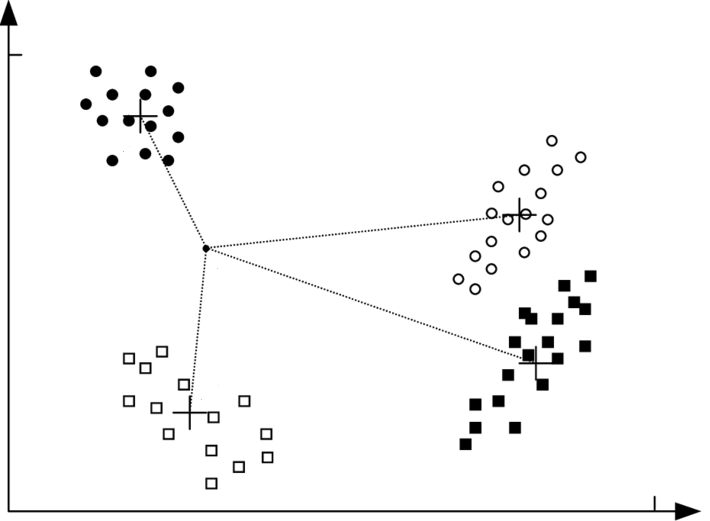
\includegraphics[scale=0.9]{images/nm_example.png}
	\caption{Przykład działania algorytmu k najbliższych sąsiadów \cite{bib2}}
	\label{algorytm_nm}
\end{figure}

 
\indent Dla każdej klasy wyznaczany jest punkt średni, na podstawie którego dokonywana będzie klasyfikacja próbki testującej (czarny punkt w centrum). Przerywane linie oznaczają drogę do centroida kolejnej klasy. 

\subsection{Algorytm k-najbliższych sąsiadów}
\indent Polega na znalezieniu k najbardziej podobnych próbek w zbiorze uczącym do obiektu testowego. Współczynnik k określa ilu sąsiadów będziemy szukać. Dla algorytmu najbliższego sąsiada wartość ta będzie równa 1. Po ustaleniu sąsiedztwa (zbiór k punktów leżących najbliżej) sprawdzamy, z której klasy danych próbek jest najwięcej. Podobieństwo obiektów badane jest przy pomocy wybranych metryk odległościowych. Dla lepszego zobrazowania działania algorytmu, poniżej znajduje się prosty przykład bazujący na wektorach w przestrzeni dwuwymiarowej. \newline
\begin{figure}[H]
	\centering
		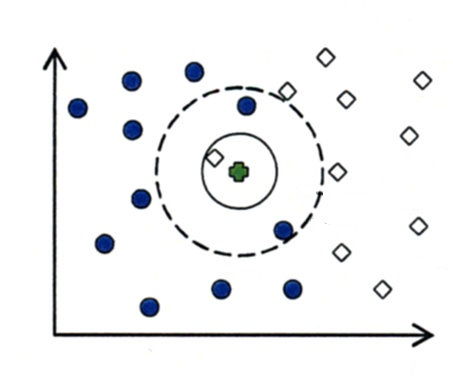
\includegraphics[scale=1]{images/knn_example.png}
	\caption{Przykład działania algorytmu k najbliższych sąsiadów \cite{bib3}}
\end{figure}

\indent Jak można zauważyć na przykładzie, klasyfikacja dla wartości parametru k równej 1 będzie przypisywała nasz obiekt testowy do klasy białej, natomiast zwiększając wielkość sąsiędztwa sytuacja się zmieni.
%---------------------------------------------------------
%					Część Trzecia
%---------------------------------------------------------
\section{Informacja o środowisku implementacyjnym}

\indent Badania zostały przeprowadzone przy pomocy języka Python w wersji 3.6. Do stworzenia rankingu cech przy użyciu kryterium Kołmogorova-Smirnova, dla każdego z parametru została użyta metoda ks\_2samp z biblioteki scipy, przyjmująca dwa wektory opisujące poszczególne klasy. Algorytmy natomiast zostały zaimplementowane z użyciem biblioteki sklearn wykorzystując metody KNeighborsClassifier oraz NearestCentroid zwracające wybrany klasyfikator. Na jego podstawie trenowany był zbiór uczący przy pomocy metody fit, a następnie przy pomocy funkcji predict przyjmującej jako parametr zbiór testowy dokonywana była diagnoza. Otrzymane wartości klasyfikacji porównano z rzeczywistym stanem badanego obiektu wykorzystując opisane w kolejnej części metryki klasyfikacji.


%---------------------------------------------------------
%					Część czwarta
%---------------------------------------------------------
\section{Opis badań eksperymentalnych}
\indent W badaniu zostały porównane algorytmy opisane w punkcie 2 niniejszej pracy. Dodatkowo każdy z nich został uruchomiony z różnymi parametrami wejściowymi tj. rodzaj metryki klasyfikacji, sposób mierzenia odległości pomiędzy próbkami, normalizacja wektora cech, jego długość czy w przypadku algorytmu najbliższego sąsiada wielkość parametru k. Porównanie różnych wariantów tych wartości zostało umieszczone w kolejnym punkcie tej pracy. Poniżej przedstawiono szczegóły dotyczące przeprowadzonych badań.\\

\subsection{Parametry klasyfikacji}
W tabeli \ref{parametry_klasyfiacji} zostały przedstawione parametry wejściowe wykorzystywane w procesie klasyfikacji.
\begin{table}[H]
\captionof{table}{Parametry klasyfikacji} 
\label{parametry_klasyfiacji}
	\begin{tabular}{|p{0.3\linewidth}|p{0.64\linewidth}|}%{|l|l|}
	\hline\centering
	Rodzaj parametru 	& Testowane wartości 		\\ \hline\centering
	Metryki klasyfikacji	& accuracy, balanced, copen kappa \\ \hline\centering
	Algorytm	& NM, 1-NN, 5-NN, 9-NN \\ \hline\centering
	Metryka odległości	& euklides, manhatan \\ \hline\centering
	Wektor cech	& z normalizacją, bez normalizacji \\ \hline\centering
	Liczba cech	& Liczby naturalne z przedziału $<1;30>$ \\ \hline
	\end{tabular}
\end{table}

\centerline{\textbf{Opis wykorzystanych metryk klasyfikacji \cite{bib4}: }}
Podczas omawiania metryk, do lepszego zrozumienia ich działania wprowadzony został przykład, który przeliczany jest dla każdej z metryk. Funkcje te, do wyznaczenia dokładności działania klasyfikatora wykorzystują jako pierwszy parametr zbiór etykiet zgodny z stanem rzeczywistym  obiektów ($y_{true}$) oraz zbiór przewidywanych klas przypisywanych przez klasyfikator ($y_{pred}$). Poniżej znajdują się przykładowe oba zbiory wykorzystane w dalszych rozważaniach. \\
\begin{center}
$ y_{true} = [A, B, A, A, B, A]$ \\
$ y_{pred} = [A, B, A, A, A, B]$ \\
\end{center}
\textbf{Accuracy} - porównuje przewidywane wartości klasyfikacji z ich rzeczywistym stanem, diagnoza jest zgodna tylko w przypadku dokładnie przewidzianego wyniku. W naszym przykładzie, składającym się z 6 obiektów, 4 klasyfikator przypisał prawidłowo. W związku z tym jego dokładność przy pomocy tej metryki będzie wynosiła w przybliżeniu 0,66.
\begin{center}
$ score_{accuracy} = 0,(66) $
\end{center}
\textbf{Balanced} - metryka wykorzystywana przy niezbalansowanych zbiorach danych. Jest zdefiniowana jako średnia poprawnych wyników uzyskana dla poszczególnych klas. W przykładzie powyżej mamy dwie klasy A (4 obiekty) i B (2 obiekty). Do klasy A poprawnie zaklasyfikowano 3  obiekty, co daje nam wynik poprawności 0,75 natomiast dla klasy B jedną próbkę w związku z tym poprawność wynosi 0,5. Ogólny wynik klasyfikatory jest średnią uzyskanych wyników:
\begin{center}
$ score_{balanced} = \frac{0,5+0,75}{2} = 0,625 $
\end{center}
\textbf{Cohen kappa} - ogólnie jest to metryka, która porównuje zgodność wyników różnych stron tzw. sędziów (oceniających przynależność do danej klasy). W naszym przypadku będzie opierała się ona o macierz konfuzji inaczej pomyłek. Jest ona narzędziem stosowanym do oceny jakości klasyfikacji. Polega na zestawieniu otrzymanych wyników z rzeczywistością w formie tabeli. Dla naszego dwu klasowego problemu rozpoznawania rozpatrywanego w niniejszej pracy będzie miała ona kształt:
\begin{table}[H]
\begin{tabular}{cccll}
\cline{1-3}
\multicolumn{1}{|c|}{}                          & \multicolumn{1}{c|}{\cellcolor[HTML]{FCFF2F}{\color[HTML]{333333} M}} & \multicolumn{1}{c|}{\cellcolor[HTML]{FCFF2F}{\color[HTML]{333333} B}} &  &  \\ \cline{1-3}
\multicolumn{1}{|c|}{\cellcolor[HTML]{34FF34}M} & \multicolumn{1}{c|}{Tm}                                               & \multicolumn{1}{c|}{Fm}                                               &  &  \\ \cline{1-3}
\multicolumn{1}{|c|}{\cellcolor[HTML]{34FF34}B} & \multicolumn{1}{c|}{Fb}                                               & \multicolumn{1}{c|}{Tb}                                               &  &  \\ \cline{1-3}
                                                &                                                                       &                                                                       &  & 
\end{tabular}
\end{table}

Zielonym kolorem oznaczone są etykiety mówiące o rzeczywistej klasie, natomiast żółty przedstawia etykiety wyników klasyfikacji. Liczby na przekątnej oznaczają prawidłowe przypisanie do klasy. Tm oznacza prawidłowe przypisane próbek do klasy raka złośliwego, Fm natomiast nieprawidłowe przypisanie obiektów z klasy złośliwej do klasy raka łagodnego. Podobnie sytuacja wygląda w przypadku klasy B. W przypadku naszego przykładu znajdującego się w tym punkcie powyżej, macierz wraz z uzupełnionymi wartościami wygląda następująco.

\begin{table}[H]
\begin{tabular}{cccll}
\cline{1-3}
\multicolumn{1}{|c|}{}                          & \multicolumn{1}{c|}{\cellcolor[HTML]{FFFFFF}{\color[HTML]{333333} A}} & \multicolumn{1}{c|}{\cellcolor[HTML]{FFFFFF}{\color[HTML]{333333} B}} &  &  \\ \cline{1-3}
\multicolumn{1}{|c|}{\cellcolor[HTML]{FFFFFF}A} & \multicolumn{1}{c|}{3}                                                & \multicolumn{1}{c|}{1}                                                &  &  \\ \cline{1-3}
\multicolumn{1}{|c|}{\cellcolor[HTML]{FFFFFF}B} & \multicolumn{1}{c|}{1}                                                & \multicolumn{1}{c|}{1}                                                &  &  \\ \cline{1-3}
                                                &                                                                       &                                                                       &  & 
\end{tabular}
\end{table}

Do obliczenia współczynniku dokładności metryki Cohen cappa wykorzystywany jest następujący wzór.
\begin{center}
$ k = \frac{p_{0}-p_{e}}{1-p_{e}}$ \\
\end{center}

I tak $p_{0}$ jest prawdopodobieństwem poprawnie przypisanych obiektów, w tym przykładzie było ich 4, co daje ułamek 0,(66). Natomiast $p_{e}$ składa się z prawdopodobieństwa przypisania do klasy A przez obie strony (sędziów, w naszym przypadku klasyfikatora i rzeczywistości). Wynik tego działania znajduje się poniżej wraz z obliczoną poprawnością.
\begin{center}
$ p_{e} = p_{A} + p_{B} $ \\
$ p_{A} = \frac{4}{6} * \frac{4}{6} = \frac{4}{9}$ \\
$ p_{B} = \frac{2}{6} * \frac{2}{6} = \frac{1}{9}$ \\
$ p_{e} = \frac{5}{9} $ \\

$ k = \frac{\frac{2}{3}-\frac{5}{9}}{1 - \frac{5}{9}} = \frac{\frac{1}{9}}{\frac{4}{9}} = 0,25 $ \\
\end{center}

\indent Pozostałe parametry klasyfikacji zostały wyjaśnione we wcześniejszych rozważaniach pracy bądź zostały pominięte przez autorów pracy w związku z ich małym stopniem skomplikowania.
\newline
\subsection{Badania}
\indent  Przeprowadzenie badań odbyło się z wykorzystaniem 5 razy powtarzanej metody 2-krotnej walidacji krzyżowej. Wszystkich pacjentów losowo podzielono na wspominany zbiór uczący oraz testujący. Następnie uruchomiono na testowanych obiektach poszczególne algorytmy zmieniając kolejno wyżej wymienione rodzaje parametrów. Dodatkowo zmieniano liczbę cech w wektorze opisującym próbki od wartości 1 aż do 26 (4 próbki odpadły po wykonaniu rankingu cech). Dla każdej konfiguracji zapisano wyniki. Po wykonanych badaniach zamieniono zbiory. Zbiór uczący stał się testującym i na odwrót, zbiór testujący uczącym. Po raz kolejny wykonano badania a wyniki zapisano. Proces ten, rozpoczynający się od losowania zbioru powtórzono pięciokrotnie, co sprawiło, że osiągnięte wyniki będą bardziej wiarygodne.
\newline
\indent W związku z dużą liczbą danych wynikających z ilością zmiennych parametrów, badania nie są przeprowadzone dla wszystkich możliwych konfiguracji (zmniejszyłaby się czytelność i utrudniłoby to analizę wyników). Najpierw przeprowadzone zostało porównanie metryk sprawdzających poprawność diagnoz, biorąc pod uwagę wszystkie zaimplementowane algorytmy. Następnie dla najskuteczniejszej metryki przetestowano algorytmy, sprawdzając osiągane przez nie dokładności. Dla najlepszej konfiguracji wspomnianych wyżej parametrów porównano zostały metryki odległości, a na koniec przyrównano wyniki osiągane z normalizacją wektora cech poszczególnych pacjentów oraz bez normalizacji. Osiągnięte rezultaty oraz wnioski z nich wynikające przedstawiono w dalszej części pracy.

%---------------------------------------------------------
%					Część piąta
%---------------------------------------------------------
\section{Wyniki}
\newpage 
\begin{figure}[H]
	\centering
	\captionof{table}{Wyniki pomiarowe wykonane na podstawie zaimplementowanych algorytmów}
		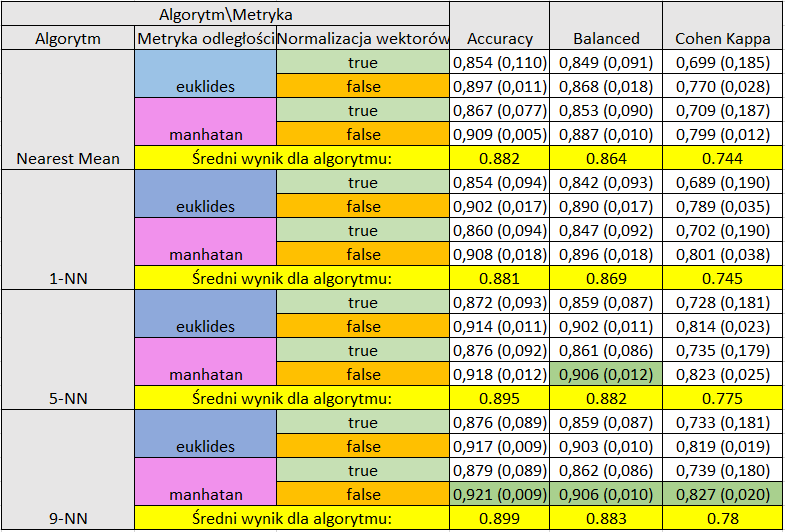
\includegraphics[scale=0.75]{images/ogolna_tabela.png}
\end{figure}

% Porownanie metryk 

%-------------------------EUKLIDES--------------------------
\subsection{Porównanie metryk klasyfikacji}
\subsubsection{Euklides}
\begin{figure}[H]
	\centering
	\captionof{table}{Porównanie metryk dla algorytmu 9 najbliższych sąsiadów z normalizacją wektorów}
		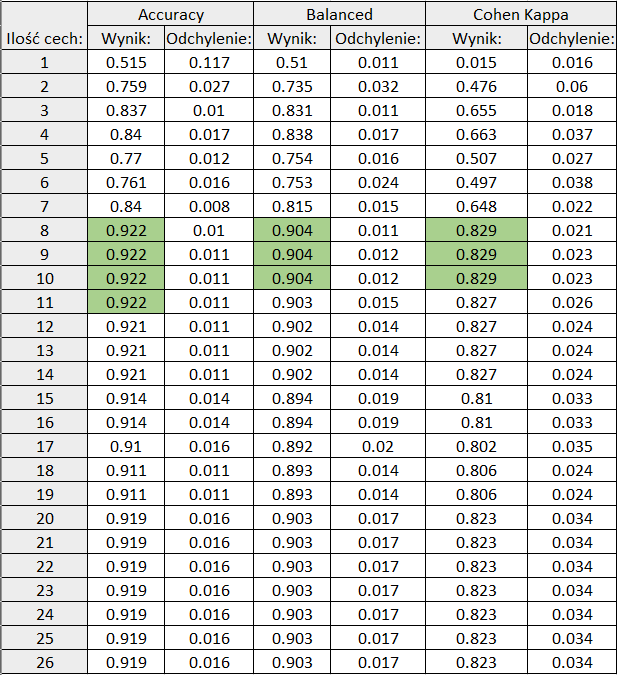
\includegraphics[scale=0.9]{images/metrics/9nn_euklides_norm_tab.png}
\end{figure}
\begin{figure}[H]
	\centering
	\captionof{table}{Porównanie metryk dla algorytmu 9 najbliższych sąsiadów bez normalizacji wektorów}
		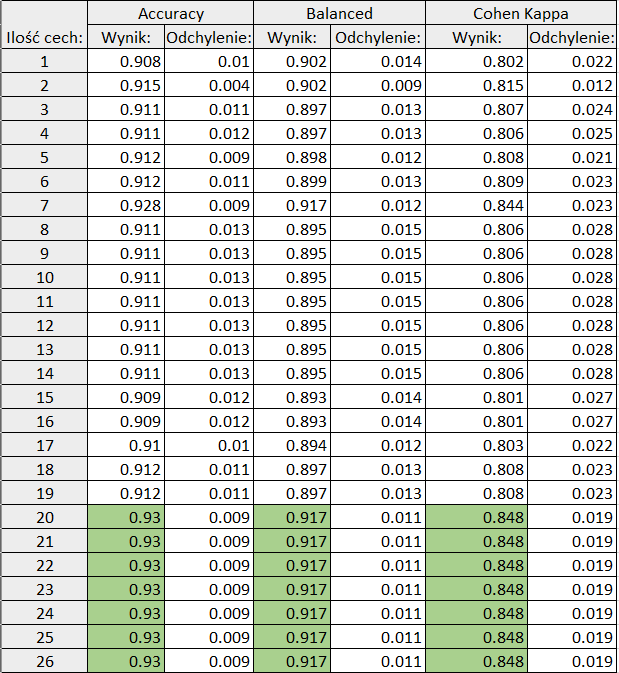
\includegraphics[scale=0.9]{images/metrics/9nn_euklides_beznorm_tab.png}
	
\end{figure}

\begin{figure}[H]
	\centering
		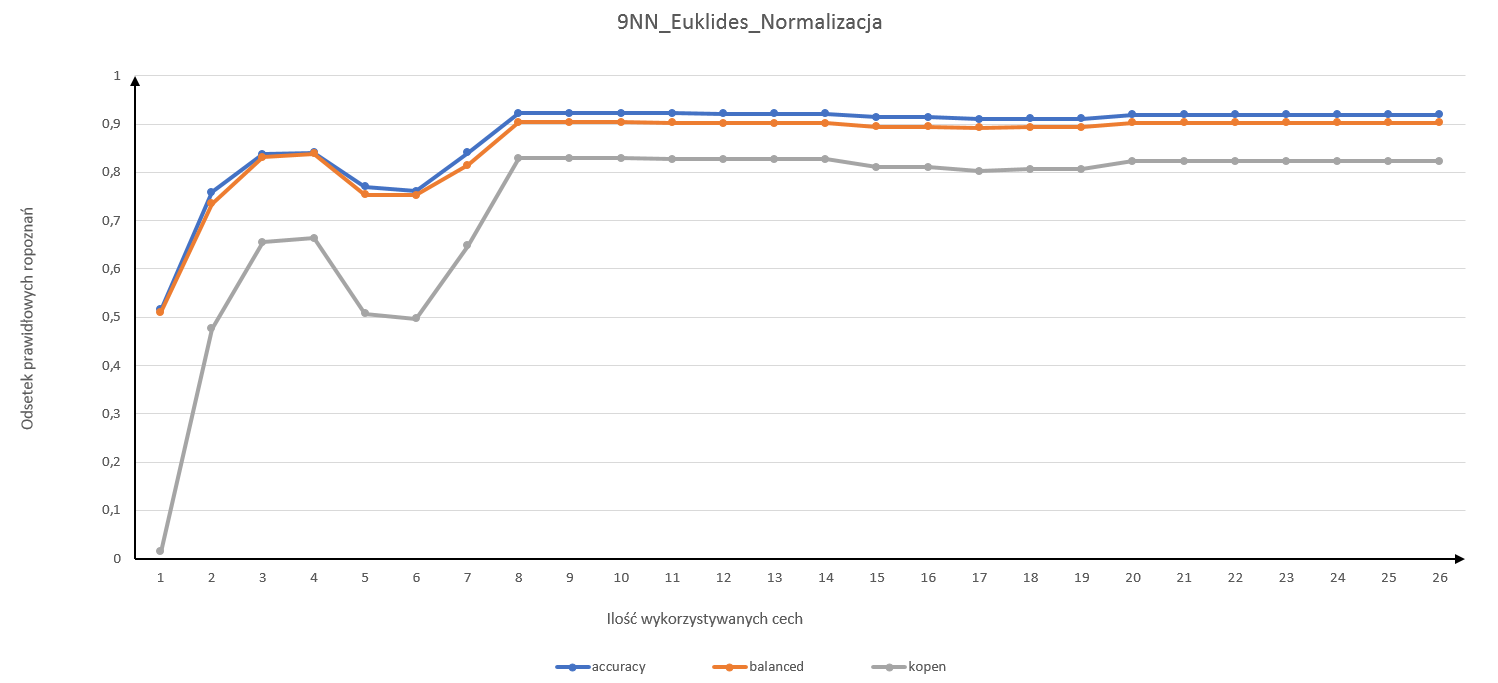
\includegraphics[scale=0.66]{images/metrics/9nn_euklides_norm.png}
	\caption{Porównanie metryk dla algorytmu 9 najbliższych sąsiadów z normalizacją wektorów}
\end{figure}
\begin{figure}[H]
	\centering
		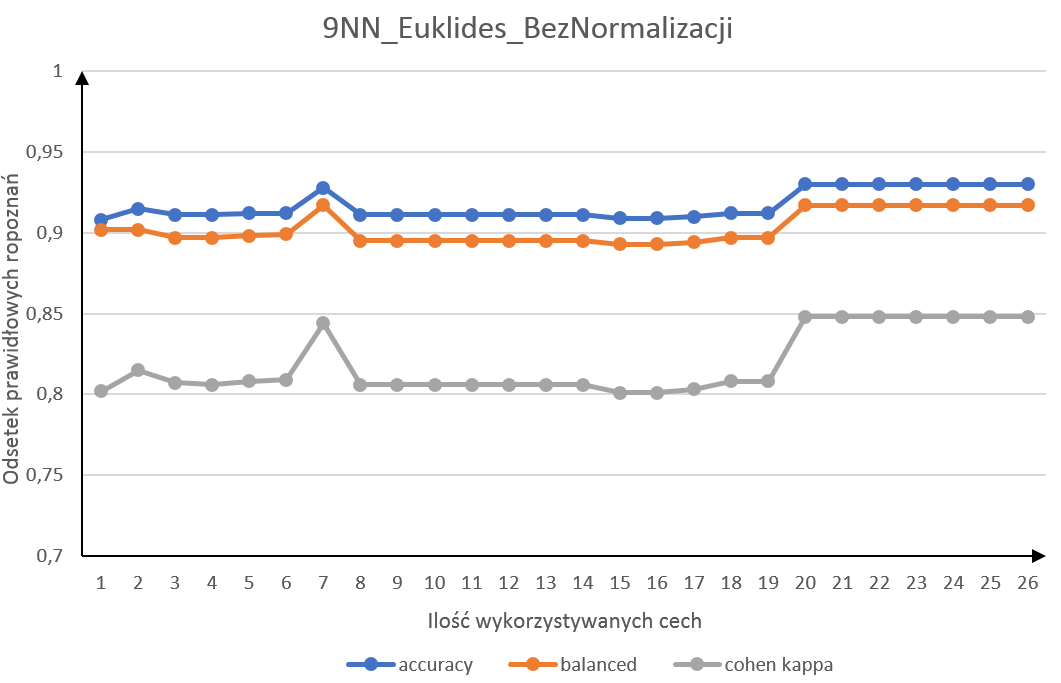
\includegraphics[scale=0.66]{images/metrics/9nn_euklides_beznorm.png}
	\caption{Porównanie metryk dla algorytmu 9 najbliższych sąsiadów bez normalizacji wektorów}
\end{figure}
%-------------------------EUKLIDES--------------------------

\subsubsection{Manhatan}
%-------------------------MANHATAN--------------------------
\begin{figure}[H]
	\centering
	\captionof{table}{Porównanie metryk dla algorytmu 9 najbliższych sąsiadów z normalizacją wektorów}
		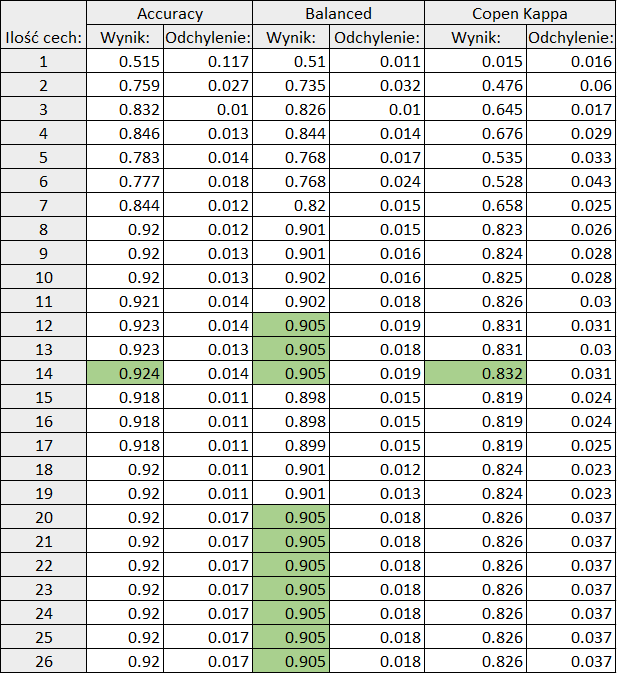
\includegraphics[scale=0.9]{images/metrics/9nn_manhatan_norm_tab.png}
	
\end{figure}
\begin{figure}[H]
	\centering
	\captionof{table}{Porównanie metryk dla algorytmu 9 najbliższych sąsiadów bez normalizacji wektorów}
		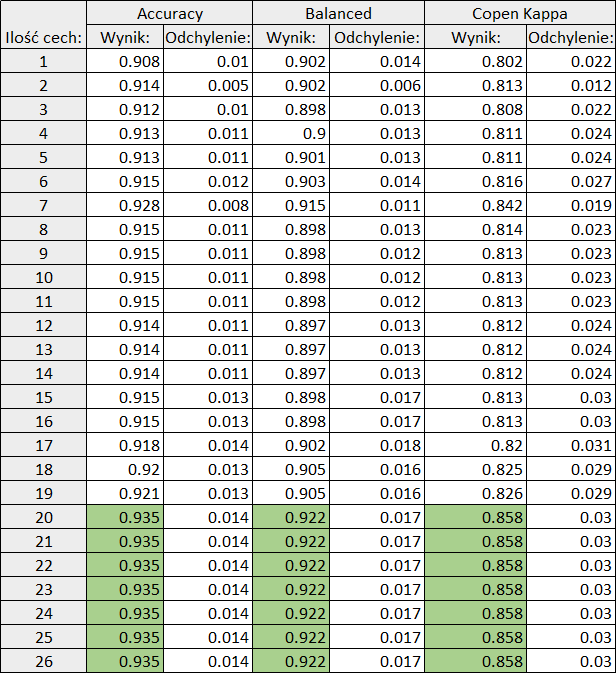
\includegraphics[scale=0.9]{images/metrics/9nn_manhatan_beznorm_tab.png}
	
\end{figure}
\begin{figure}[H]
	\centering
		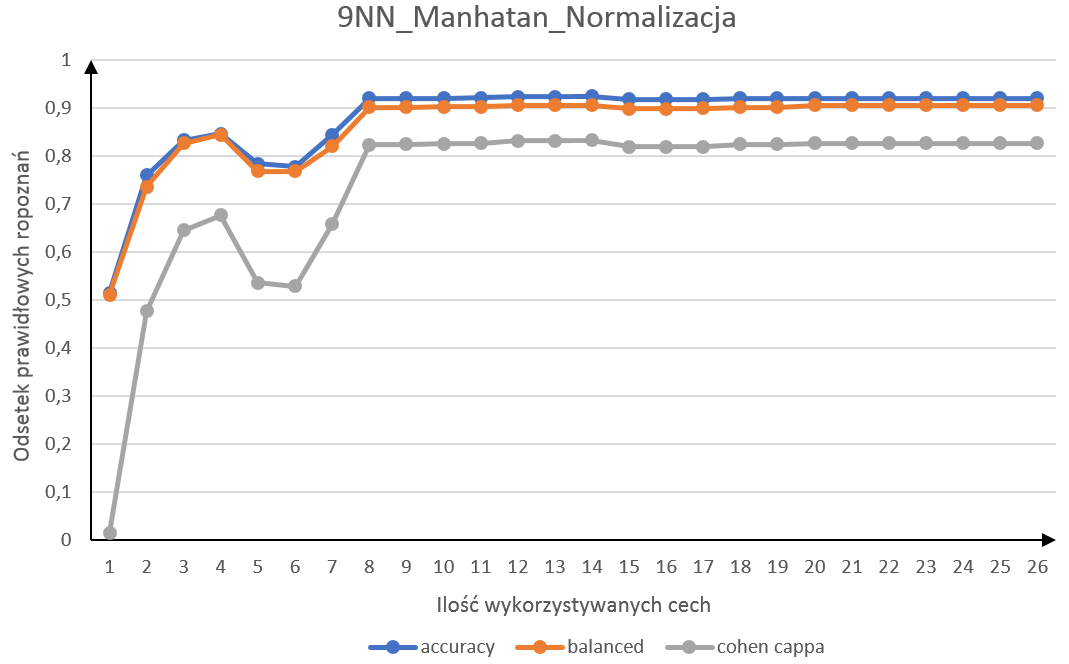
\includegraphics[scale=0.66]{images/metrics/9nn_manhatan_norm.png}
	\caption{Porównanie metryk dla algorytmu 9 najbliższych sąsiadów z normalizacją wektorów}
\end{figure}
\begin{figure}[H]
	\centering
		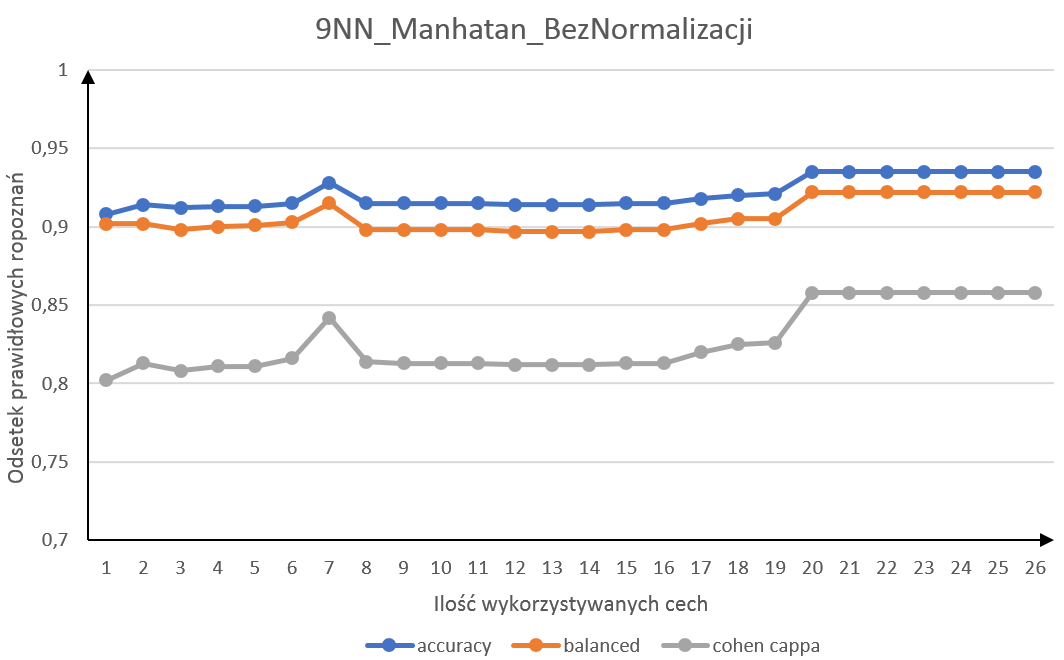
\includegraphics[scale=0.66]{images/metrics/9nn_manhatan_beznorm.png}
	\caption{Porównanie metryk dla algorytmu 9 najbliższych sąsiadów bez normalizacji wektorów}
\end{figure}
%-------------------------MANHATAN--------------------------
\subsection{Porównanie algorytmów}
%Porownanie algorytmów

\begin{figure}[H]
	\centering
	\captionof{table}{Porównanie algorytmów dla metryki odległościowej \textit{Euklides} z normalizacją wektorów}
		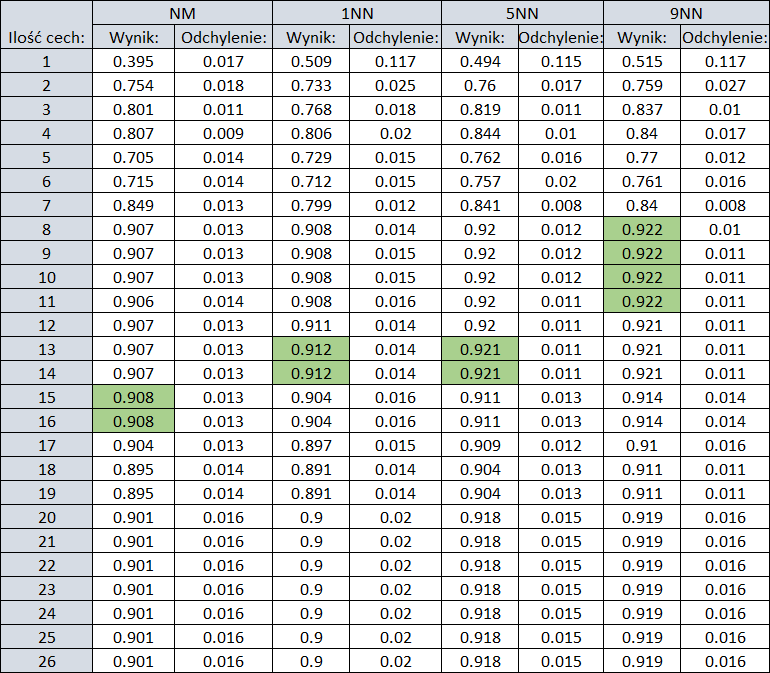
\includegraphics[scale=0.8]{images/algorithms/euklides_norm_tab.png}
	
\end{figure}

\begin{figure}[H]
	\centering
		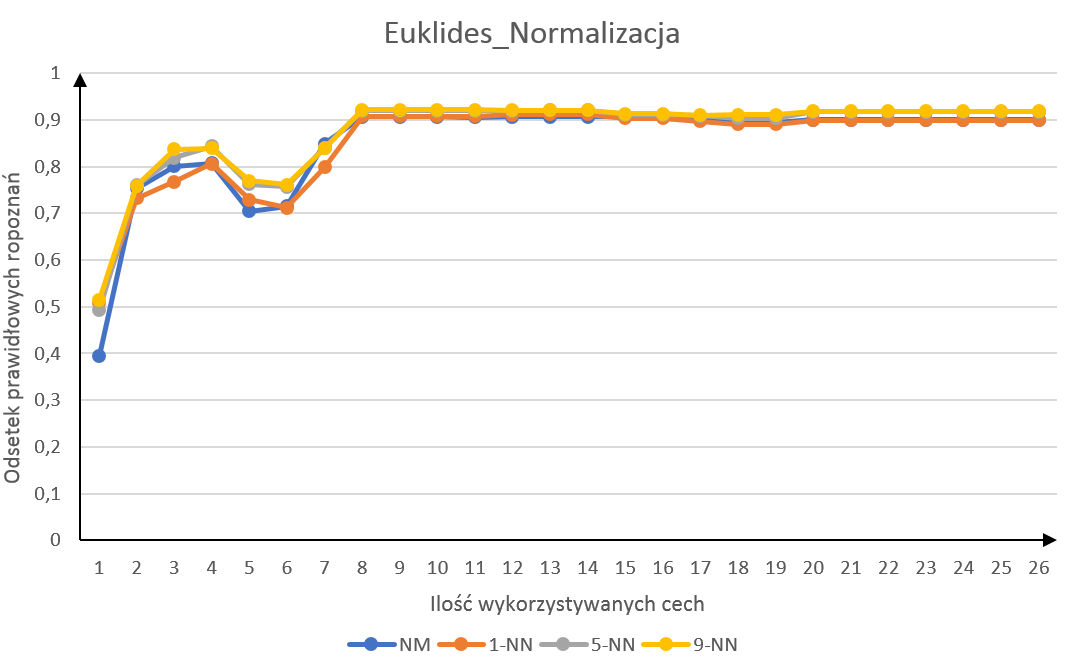
\includegraphics[scale=0.66]{images/algorithms/euklides_norm.png}
	\caption{Porównanie algorytmów dla metryki odległościowej \textit{Euklides} z normalizacją wektorów}
\end{figure}

\begin{figure}[H]
	\centering
	\captionof{table}{Porównanie algorytmów dla metryki odległościowej \textit{Manhatan} z normalizacją wektorów}
		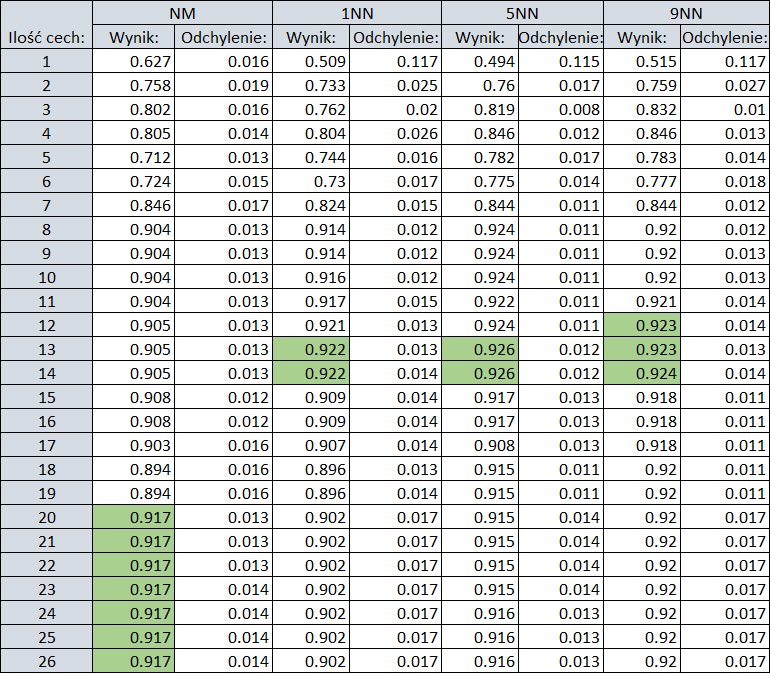
\includegraphics[scale=0.8]{images/algorithms/manhatan_norm_tab.png}
	
\end{figure}

\begin{figure}[H]
	\centering
		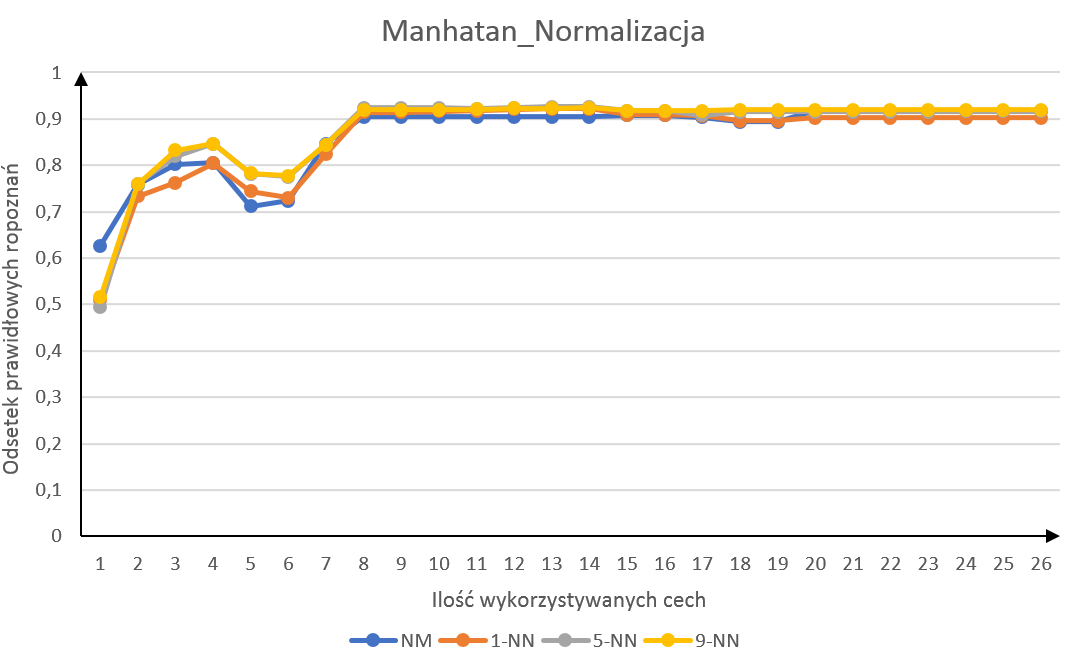
\includegraphics[scale=0.66]{images/algorithms/manhatan_norm.png}
	\caption{Porównanie algorytmów dla metryki odległościowej \textit{Manhatan} z normalizacją wektorów}
\end{figure}

\begin{figure}[H]
	\centering
	\captionof{table}{Porównanie algorytmów dla metryki odległościowej \textit{Euklides} bez normalizacji}
		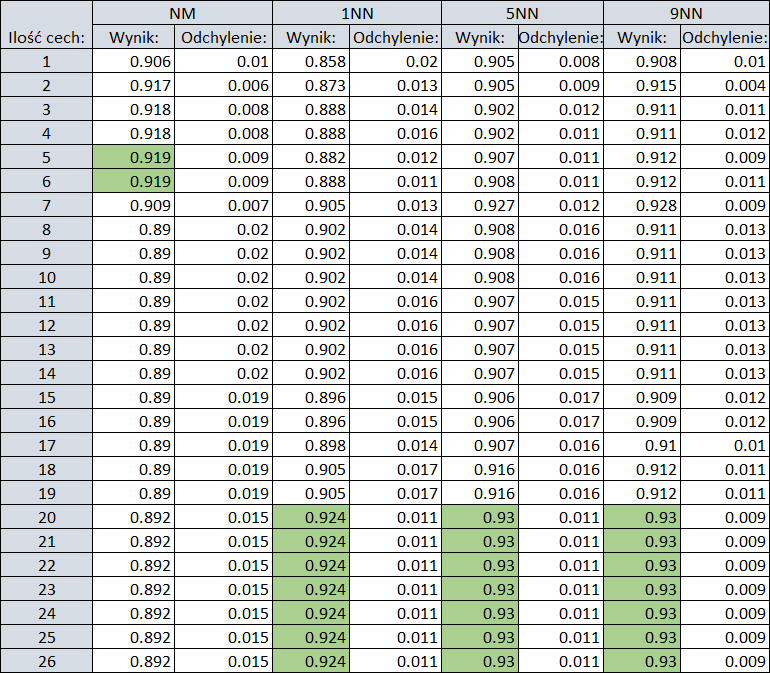
\includegraphics[scale=0.8]{images/algorithms/euklides_beznorm_tab.png}
	
\end{figure}
\begin{figure}[H]
	\centering
		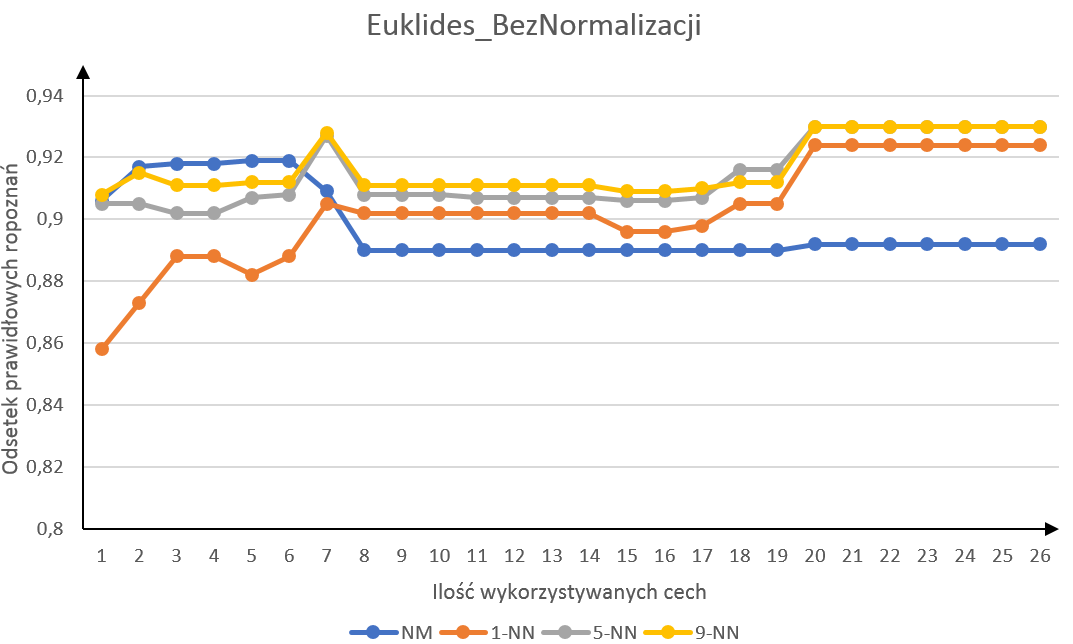
\includegraphics[scale=0.66]{images/algorithms/euklides_beznorm.png}
	\caption{Porównanie algorytmów dla metryki odległościowej \textit{Euklides} bez normalizacji wektorów}
\end{figure}

\begin{figure}[H]
	\centering
	\captionof{table}{Porównanie algorytmów dla metryki odległościowej \textit{Manhatan} bez normalizacji}
		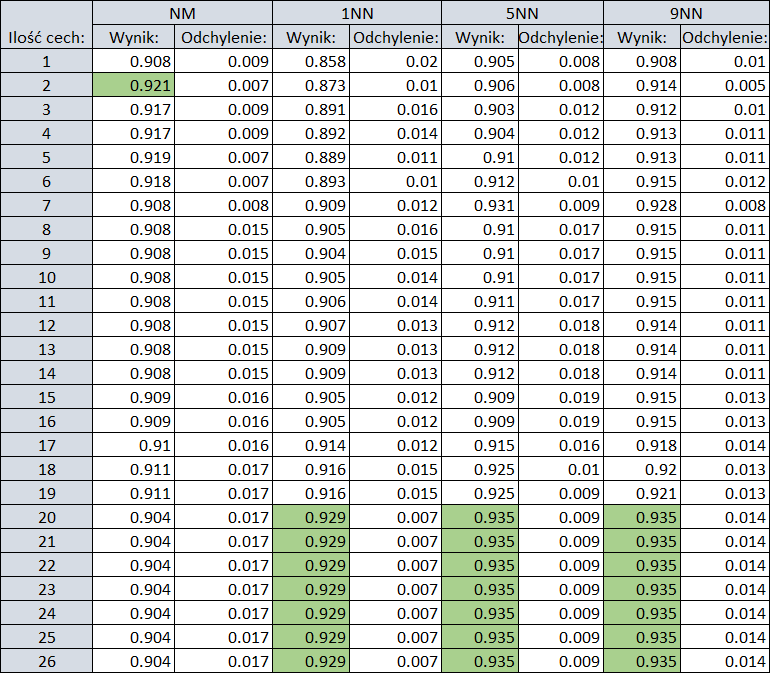
\includegraphics[scale=0.8]{images/algorithms/manhatan_beznorm_tab.png}
	
\end{figure}
\begin{figure}[H]
	\centering
		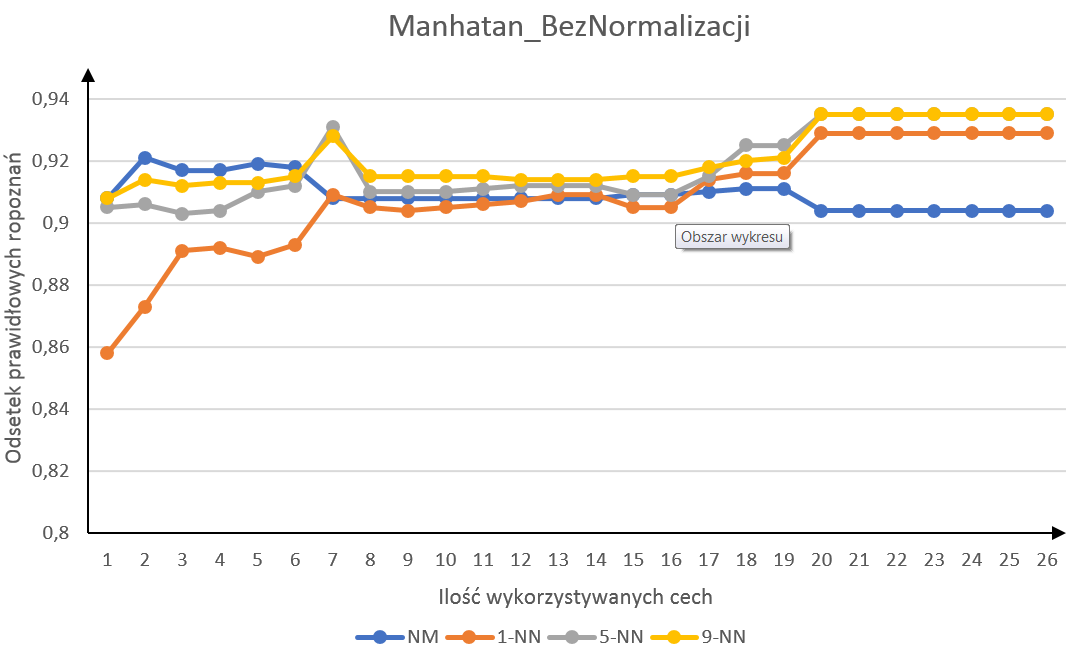
\includegraphics[scale=0.66]{images/algorithms/manhatan_beznorm.png}
	\caption{Porównanie algorytmów dla metryki odległościowej \textit{Manhatan} bez normalizacji}
\end{figure}


% Porównanie metryk odległościowych
\subsection{Porównanie metryk odległościowych}
\begin{figure}[H]
	\centering
	\captionof{table}{Porównanie metryk odległościowych i reprezentacji wektorów cech}
		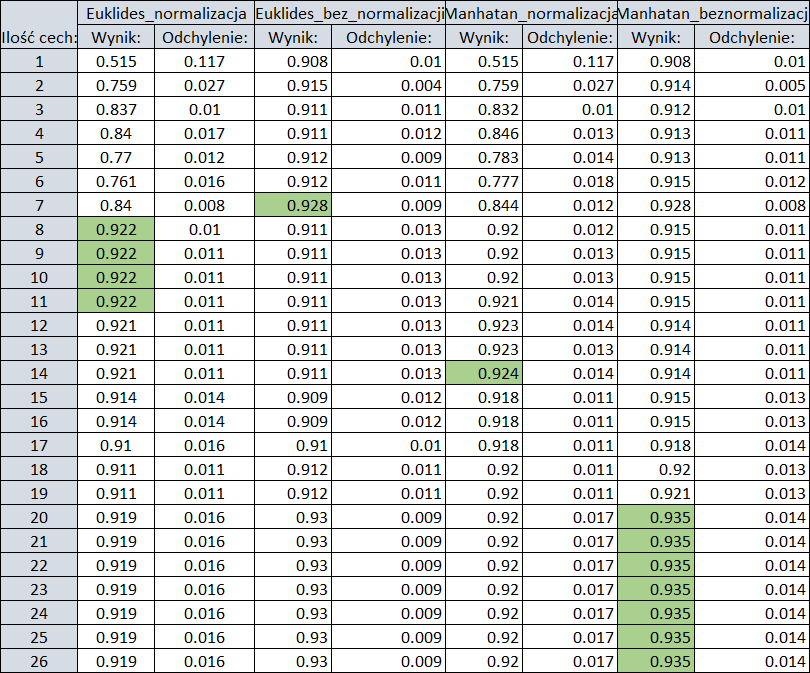
\includegraphics[scale=0.77]{images/distance_metrics/distance_metrics_tab.png}
	
\end{figure}
\begin{figure}[H]
	\centering
		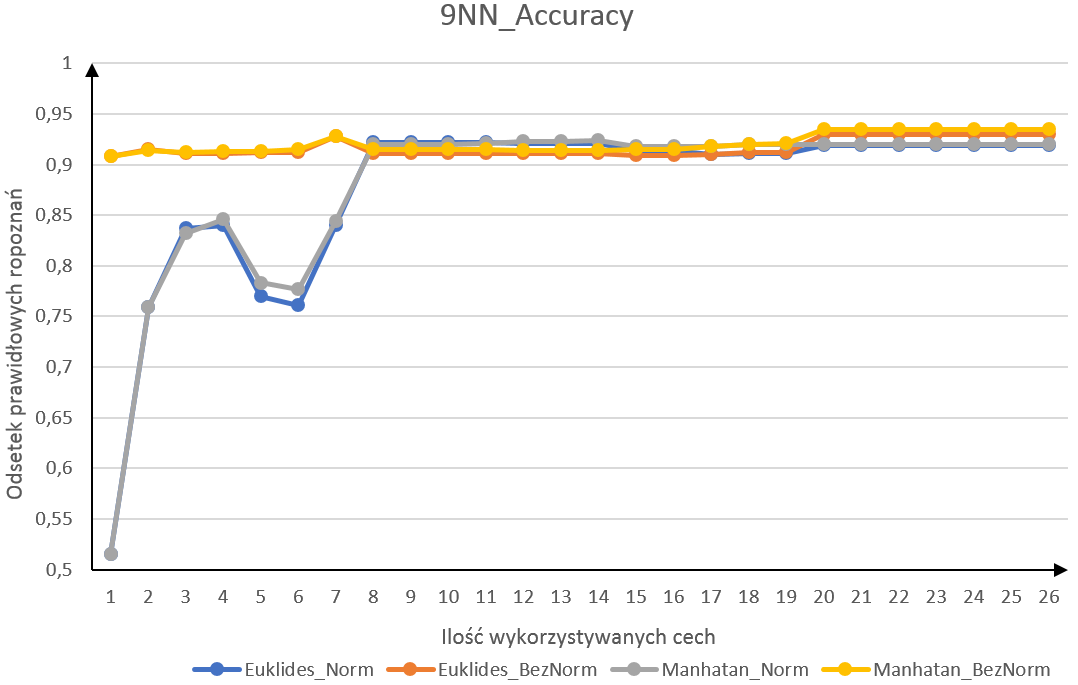
\includegraphics[scale=0.66]{images/distance_metrics/distance_metrics.png}
	\caption{Porównanie metryk odległościowych i reprezentacji wektorów cech}
\end{figure}

%---------------------------------------------------------
%					Część szósta
%---------------------------------------------------------

\section{Dyskusja wyników i wnioski wynikające z badań.}

Porównanie metryk wyszło super, algorytmy śmigały aż miło. Raka diagnozowaliśmy w 90\% a w kolejnych 10\% przepisywaliśmy pacjentkom dodatkowe prywatne badanie cyckuf



\newpage
\renewcommand\refname{Bibliografia}
\addcontentsline{toc}{section}{Bibliografia} %utworzenie w spisie treści pozycji Bibliografia
\begin{thebibliography}{9}

\bibitem{bib1}  https://en.wikipedia.org/wiki/Nearest\_centroid\_classifier

[Dostęp: 10.05.2019]

\bibitem{bib2}  https://www.researchgate.net/figure/Schematic-diagram-illustrating-the-classification-of-pixel-4-using-minimum-distance\_fig3\_294596525

[Dostęp: 10.05.2019]

\bibitem{bib3}  %\https://www.researchgate.net/figure/K-nearest-neighbor-classifier-KNN-for-k-1-und-k-3_fig6_224345777

[Dostęp: 10.05.2019]

\bibitem{bib4}  %https://scikit-learn.org/stable/modules/model_evaluation.html
[Dostęp: 11.05.2019]

\end{thebibliography}

\end{document}


